\documentclass[lettersize,journal]{IEEEtran}

\usepackage{amsmath,amsfonts}
\usepackage{array}
\usepackage[caption=false,font=normalsize,labelfont=sf,textfont=sf]{subfig}
\usepackage{textcomp}
\usepackage{stfloats}
\usepackage{url}
\usepackage{graphicx}
\usepackage{cite}
\usepackage{xcolor}
\usepackage{balance}
\usepackage{booktabs}
\usepackage{tabularx}
\usepackage{ragged2e}
\usepackage{float}
\usepackage{algorithm}
\usepackage{algpseudocode}



\newcolumntype{Y}{>{\RaggedRight\arraybackslash}X}
\newcolumntype{P}[1]{>{\RaggedRight\arraybackslash}p{#1}}

\newcommand{\status}[1]{\textbf{#1}}

\begin{document}
	\title{Vision-Based Orientation Estimation and Correction for the
	SOFIA Modular Kinetic Surface}
	
	\author{
		Marco Heimdal Castro Magaña, Alejandro Amador Franco, Karen Alejandra Guevara Vasquez, María Alicia Vela Contreras, Juan Pablo Contreras Quiñones,
		Jorge A. Lizarraga, Luis E. González-Jiménez, Luis F. Luque-Vega
		
		\thanks{The authors are with the Department
			of Electronics and Computer Systems,
			ITESO, Tlaquepaque 45604, Jalisco, Mexico.}
	}
	
	
	\markboth{Laboratory for the Development of Technological Solutions}
	{Vision-Based Orientation Estimation and Correction for SOFIA}
	
	\maketitle
	
	
	
\begin{abstract}
    \linelabel{ln:abstract}The SOFIA modular kinetic surface consists of 16 electromechanical modules arranged in a honeycomb configuration, each providing two rotational degrees of freedom through servomotors. 
	Accurate orientation control is essential for coordinated movement, as differences between commanded and actual platform orientations may affect the system's performance. This work presents a vision-based orientation 
	estimation and correction system that uses a neural network to evaluate the physical inclination of the hexagonal platforms. The proposed approach integrates visual perception with the existing embedded control architecture, 
	consisting of an ESP32-C3 microcontroller and PCA9685 PWM drivers. The estimated orientation is compared with the desired reference to determine angular deviations and generate corrective commands for the servomotors. 
	This external feedback mechanism enables the system to adjust platform orientation based on visual measurements rather than relying exclusively on commanded servo positions. Experimental evaluation is being developed to quantify angular estimation accuracy with $0.204^\circ$ mean angular error and $3.3^\circ$ maximum error, 
	residual orientation error, and correction performance under controlled operating conditions. The study aims to assess the feasibility of visual feedback for improving orientation control in modular kinetic surfaces.
\end{abstract}

	
	\begin{IEEEkeywords}
		\linelabel{ln:keywords}Visual feedback control, orientation estimation, neutral networks, computer vision, modular robotics, kinetic surfaces.
	\end{IEEEkeywords}
	
	
	\section{Introduction}
	
	\label{sec:intro}
	
	\IEEEPARstart{S}{OFIA} \linelabel{ln:intro1}is a modular robotic installation composed of 16
	mechatronic units arranged in a two-dimensional honeycomb configuration, with each
	unit providing two rotational degrees of freedom actuated by servomotors. The
	system aims to achieve coordinated control of the multiple actuators while
	enabling interaction through static and dynamic human gestures. For this
	purpose, SOFIA integrates embedded control, inter-module communication, and an
	external computer vision system for gesture recognition.
	
	\linelabel{ln:intro-cap}The SOFIA system requires the
	integration of mechanical actuation, servo control, embedded processing, and
	communication subsystems. \linelabel{ln:intro-32}Since each of the 16 units uses two servomotors, the
	complete demonstrator requires the coordinated control of 32 actuators and the
	generation of multiple PWM signals. The embedded controller must coordinate
	the desired actuator positions, while the communication architecture should
	support the future integration of additional SOFIA modules without
	significantly increasing wiring and control complexity. This work proposes a vision-based closed loop angular misalignment diagnosis for 16 modules with two-degree-of-freedom each.
	
	\subsection{Problem Statement and Research Question}
	A SOFIA module consists of 16 hexagonal plates arranged in a honeycomb configuration, where each plate can tilt in two rotational directions actuated by low-cost micro-servomotors \cite{sofia_architecture}. These actuators commonly operate with gear backlash, mechanical wear, or accidental manual contact, and without external joint feedback these servo motors can introduce angular misalignment across the surface. Instrumenting all 16 units (32 degrees of freedom) with dedicated physical angle sensors would increase wiring complexity, moving mass, and hardware cost.
	
	To address this limitation, this work investigates the following research question: \textit{Can the two tilt angles of all 16 hexagonal plates be accurately estimated from a single overhead camera to classify each unit without per-module angle sensors?} This encompasses three primary objectives: (1) designing an embedded PCB integrating an ESP32-C3 microcontroller, dual PCA9685 PWM drivers, and RS-485 interfaces to coordinate the 32 actuators. (2) integrating the diagnosis pipeline onto the physical SOFIA module using an overhead camera, four coplanar ArUco markers, and sim-to-real fine-tuning. (3) integrating state-machine execution with real-time gesture recognition.
	\begin{table*}[!t]
		\centering
		\caption{Comparative matrix of related shape-changing interface systems}
		\label{tab:related_work_matrix}
		\scriptsize
		
		\setlength{\tabcolsep}{3pt}
		\renewcommand{\arraystretch}{1.1}
		
		\begin{tabularx}{\textwidth}
			{@{}P{2.2cm} P{3cm} P{3cm} P{4cm} Y@{}}
			
			\toprule
			Reference & Method / technology & Metric / focus & Main result & Gap with respect to SOFIA \\
			\midrule
			
			Relief \cite{leithinger2010relief} &
			Array of 120 motorized pins, scalable low-cost control &
			Actuation density, hardware/software scalability &
			Continuous surface capable of rendering and animating 3D shapes, with per-pin input sensing &
			Translational actuation only (1 DOF per pin); no independent rotation per unit \\
			
			inFORM \cite{follmer2013inform} &
			Pin-based shape display on a pre-existing platform &
			Dynamic physical affordances and constraints, object manipulation &
			Real-time direct-touch interaction and physical rendering of content &
			Same translational limitation as Relief; centralized architecture, not modular per unit \\
			
			TRANSFORM \cite{ishii2015transform} &
			Three large-scale pin displays, kinetic energy as input &
			Aesthetic transformation from static furniture to dynamic system &
			Over one thousand pins coordinated in real-time wave motion &
			Installation-scale system; no per-module orientable control or distributed communication between units \\
			
			PneUI \cite{yao2013pneui} &
			Pneumatically actuated multi-layer soft composite materials &
			Integrated input sensing and shape output in the material itself &
			Four functional applications (phicons, mobile, case, lamp) with controllable shape change &
			Soft/pneumatic actuation, not discrete rotational motion; difficult to scale to precise angular control \\
			
			LineFORM \cite{nakagaki2015lineform} &
			Serial chain of one-DOF servo actuators &
			Line/curve-based interaction affordances &
			Cord, mobile, and body-constraint interfaces through line-shaped actuation &
			Serial (chain) configuration, not a two-dimensional array; 1 DOF per unit, not 2 \\
			
			ChainFORM \cite{nakagaki2016chainform} &
			Identical modules with servo, touch sensing, visual output and embedded processing &
			Hardware modularity and reconfigurability &
			Modular, reconfigurable platform with rich per-module I/O &
			Modularity demonstrated, but still a linear chain, not a 2D array with 2 DOF per node \\
			
			\bottomrule
			
		\end{tabularx}
	\end{table*}
	
	\subsection{Related shape-changing interface systems}
	\linelabel{ln:rw1}Motorized arrays have been widely explored as a mechanism for generating
	dynamic physical surfaces. Relief introduced an actuated tabletop composed of
	120 individually addressable motorized pins and emphasized a scalable hardware
	and software architecture \cite{leithinger2010relief}. This concept was
	extended through inFORM, where shape actuation was employed to generate dynamic
	physical affordances and constraints and to manipulate physical objects
	\cite{follmer2013inform}. At a larger scale, TRANSFORM explored the
	transformation of static physical structures into dynamic systems driven by
	streams of data and energy \cite{ishii2015transform}. These approaches
	demonstrate the potential of coordinated arrays of actuators, although their
	architectures primarily focus on large pin-based or installation-scale physical
	surfaces.
	
	\linelabel{ln:rw2}Alternative approaches have explored different actuation principles and
	modular configurations. PneUI demonstrated shape-changing interfaces based on
	pneumatically actuated soft composite materials, integrating sensing and active
	shape output within deformable structures \cite{yao2013pneui}. In contrast,
	LineFORM investigated electromechanical shape transformation through serial
	chains of one-degree-of-freedom servo actuators
	\cite{nakagaki2015lineform}. This concept evolved toward greater hardware
	modularity in ChainFORM, where identical modules incorporate motor actuation,
	sensing, visual output, and embedded processing
	\cite{nakagaki2016chainform}. These systems highlight modularity and
	distributed actuation as relevant design characteristics for reconfigurable
	physical interfaces.
	
	\linelabel{ln:rw-tab}The main technological characteristics and differences identified among the
	reviewed shape-changing interfaces are summarized in
	Table~\ref{tab:related_work_matrix}.
	
	\linelabel{ln:gap}In contrast to the reviewed shape-changing interfaces, SOFIA combines a
	two-dimensional honeycomb arrangement with two rotational degrees of freedom
	per unit. Unlike pin-based displays, which predominantly constrain motion to a
	single translational axis, or line-based modular systems organized as serial
	chains, each SOFIA unit can independently modify its orientation while
	remaining part of the same physical surface. This configuration introduces
	design challenges related to coordinated actuation, modularity, scalability,
	control architecture, electrical integration, and communication. Based on the
	reviewed literature, these characteristics were identified as relevant criteria
	for evaluating the technological architecture of the demonstrator.
	Table~\ref{tab:related_work_matrix} summarizes the comparative analysis of the
	reviewed systems, while Table~\ref{tab:benchmarking} contrasts SOFIA with the
	reviewed solutions using the established comparison criteria.
	
	\begin{table}[!t]
		\centering
		\caption{Benchmarking against related shape-changing systems}
		\label{tab:benchmarking}
		\scriptsize
		
		\setlength{\tabcolsep}{2pt}
		\renewcommand{\arraystretch}{1.05}
		
		\begin{tabularx}{\columnwidth}
			{@{}P{1.7cm} P{1.7cm} P{1.5cm} Y@{}}
			
			\toprule
			Solution & Configuration & DOF/ unit & Modularity / scalability\\
			\midrule
			
			inFORM \cite{follmer2013inform} &
			Pin array on fixed platform &
			1 (translational) &
			Low -- centralized control, not designed for modular expansion \\
			
			LineFORM / ChainFORM \cite{nakagaki2015lineform,nakagaki2016chainform} &
			Serial chain of modules &
			1 per module &
			Medium -- modular, but limited to a linear configuration \\
			
			PneUI \cite{yao2013pneui} &
			Pneumatic soft composite material &
			Continuous (non-discrete) &
			Low -- difficult to discretize into individually addressable nodes \\
			
			\textbf{SOFIA (proposed)} &
			2D array, honeycomb modules &
			\textbf{2 (rotational)} &
			\textbf{High -- I2C bus + RS-485 designed for future module expansion} \\
			
			\bottomrule
			
		\end{tabularx}
	\end{table}
	
	\linelabel{ln:opp}From the functional decomposition of the demonstrator and its comparison with
	the literature, several technological opportunities were identified. One is
	the development of a scalable control architecture capable of independently
	coordinating all actuators while reducing the processing load on the main
	controller. Another is the implementation of an inter-module communication
	architecture that allows multiple SOFIA modules to operate as part of a larger
	system. Additional opportunities include the implementation of
	software-defined motion limits and smoothing strategies to prevent abrupt
	servo movements and reduce mechanical stress.
	
	\linelabel{ln:focus}Based on these opportunities, this work focuses on a vision-based misalignment diagnosis methodology for the 16-unit SOFIA array, supported by an embedded electronic and gesture-control architecture. The selected hardware provides the 32-channel PWM generation, wireless telemetry, and differential inter-module communication interfaces required by the demonstrator, while the primary research contribution is the metric overhead rectification and neural-network-based angular estimation evaluated across datasets and prepared for physical module deployment. Automatic Modbus address assignment is outside the experimental scope.
	
	
	\section{Materials and Methods}
	\label{sec:methods}
	
	\linelabel{ln:materials-intro}The SOFIA kinetic surface consists of 16 electromechanical modules arranged in a honeycomb configuration, each providing two rotational degrees of freedom actuated by MG90S servomotors for a total of 32 actuators \cite{sofia_architecture,mg90s}. Rather than instrumenting individual actuators mechanically, this study evaluates the orientation of all 16 hexagonal top platforms simultaneously through an overhead computer vision pipeline.
	
	\linelabel{ln:hardware-config}The methodology is divided into three main stages: embedded hardware configuration, vision-based rectification with dataset generation in Webots, and comparative evaluation of angular estimation models. The first stage involves the selection and electrical verification of the electronic components required for 32-channel servomotor control and inter-module communication \cite{technical_session}. The second stage establishes an overhead camera calibration procedure using four coplanar ArUco markers to generate metric top-down crops ($1~\text{px} = 1~\text{mm}$) and automates the acquisition of labeled datasets in Webots. The third stage benchmarks a geometric displacement model, a lightweight convolutional neural network (CNN), and a hybrid decision rule to estimate platform tilt angles and classify each unit as \textit{OK} ($<2^\circ$), \textit{REVIEW} ($2^\circ\text{--}5^\circ$), or \textit{MISALIGNED} ($>5^\circ$).
	
	\linelabel{ln:methods-variables}The electronic architecture of the complete SOFIA system includes an ESP32-C3 microcontroller and two PCA9685 PWM drivers, which provide the 32 PWM channels required for actuator control \cite{sofia_architecture,esp32c3,pca9685}.
	
	\linelabel{ln:requirements-intro}The main electrical, communication, and mechanical requirements of the SOFIA demonstrator are summarized in Table~\ref{tab:sofia_requirements}. These requirements are based on the system architecture and the established technical verification criteria \cite{sofia_architecture,technical_session}.
	
	\begin{table}[!t]
		\centering
		\caption{SOFIA Main Requirements}
		\label{tab:sofia_requirements}
		\scriptsize
		
		\setlength{\tabcolsep}{2pt}
		\renewcommand{\arraystretch}{1.05}
		
		\begin{tabularx}{\columnwidth}
			{@{}P{2.1cm} P{2.1cm} Y@{}}
			
			\toprule
			Requirement & Specification & Verification\\
			\midrule
			
			Power &
			5 V servo supply &
			Compatible with MG90S range \\
			
			Logic voltage &
			3.3 V MCU logic &
			Required for ESP32-C3 GPIO \\
			
			Communication &
			WiFi/Bluetooth + I2C &
			Supported by ESP32-C3 \\
			
			PWM control &
			32 servo channels, 50 Hz &
			Two PCA9685 drivers required \\
			
			Mechanical &
			16 modules, 2 DOF each &
			32 servos required \\
			
			\bottomrule
			
		\end{tabularx}
	\end{table}
	
	Figure~\ref{fig:SOFIA_DIAGRAM} \linelabel{ln:sim_architecture} illustrates the system architecture and signal flow of the SOFIA demonstrator. Telemetry and motion commands are communicated wirelessly between a central host PC (equipped with an external vision camera) and the main PCB via Wi-Fi or Bluetooth protocols. Onboard processing is handled by an ESP32 microcontroller, which interfaces with two PCA9685 PWM drivers over $\text{I}^2\text{C}$ to control a total of 32 servos. Driver 1 manages channels CH1--CH16 (grey group), while Driver 2 addresses channels CH17--CH32 (blue group, labeled CH1--CH16 on the second module) across the Master Module actuator array. \linelabel{ln:interconn}Interconnectivity between boards is planned using JST-PH connectors.
	
	
	\begin{figure}[!t]
		\centering
		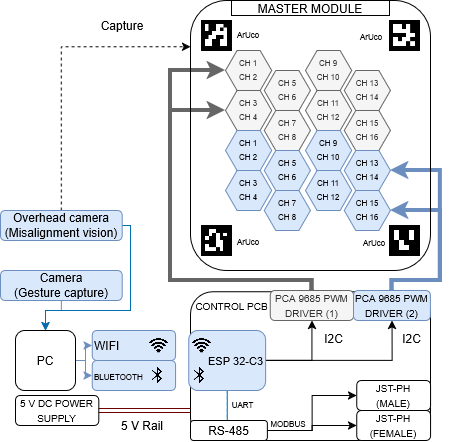
\includegraphics[width=\columnwidth]{figures/SOFIA_DIAGRAM_3}
		\caption{Block diagram describing SOFIA components and connections.}
		\label{fig:SOFIA_DIAGRAM}
	\end{figure}
	
	\subsection{ESP32-C3 Technical Analysis}
	\linelabel{ln:spec-esp-intro}The main technical specifications of the ESP32-C3 microcontroller are presented in Table~\ref{tab:esp32_specs}.
	
	\begin{table}[!t]
		\centering
		\caption{ESP32-C3 Main Specifications and Datasheet Verification \cite{esp32c3}}
		\label{tab:esp32_specs}
		\scriptsize
		
		\setlength{\tabcolsep}{2pt}
		\renewcommand{\arraystretch}{1.1}
		
		\begin{tabularx}{\columnwidth}{@{}P{1.6cm} P{1.5cm} P{2.1cm} X X@{}}
			\toprule
			\textbf{Parameter} & \textbf{Value} & \textbf{Source (Doc / Ver / Pg)} & \textbf{Justification} & \textbf{Verification} \\
			\midrule
			
			Supply Voltage & 
			3.0--3.6 V & 
			ESP32-C3 Datasheet v2.4, p. 18 & 
			Match system main power operating limits & 
			Requires regulated 3.3 V supply \\
			
			Wi-Fi & 
			802.11 b/g/n & 
			ESP32-C3 Datasheet v2.4, p. 2 & 
			Enable 2.4 GHz wireless transmission & 
			Complies; integrated 2.4 GHz subsystem \\
			
			Bluetooth & 
			BLE 5 & 
			ESP32-C3 Datasheet v2.4, p. 2 & 
			Support low-energy configuration and monitoring & 
			Complies; Bluetooth LE 5.0 supported \\
			
			Logic Level & 
			3.3 V GPIO & 
			ESP32-C3 Datasheet v2.4, p. 19 & 
			Ensure digital signal levels meet peripheral logic thresholds & 
			5 V logic cannot be applied directly without level shifting \\
			
			Boot Pins & 
			GPIO2, 8, 9 & 
			ESP32-C3 Datasheet v2.4, p. 12 & 
			Prevent unintended strapping state selection during power-up & 
			PCB design hardware strapping verification required \\
			
			Temperature & 
			Up to 105 $^\circ$C & 
			ESP32-C3 Datasheet v2.4, p. 18 & 
			Ensure reliable continuous execution under thermal load & 
			Suitable for industrial and laboratory operating environments \\
			
			\bottomrule
		\end{tabularx}
	\end{table}
	
	% Source: ESP32-C3 Datasheet, Espressif Systems. (reference included in table caption)
	
	
	\subsection{PCA9685 Technical Analysis}
	\linelabel{ln:spec-pca-intro}The specifications of the PCA9685 PWM driver are summarized in Table~\ref{tab:pca9685_specs}.
	
	\begin{table}[!t]
		\centering
		\caption{PCA9685 Main Specifications and Datasheet Verification \cite{pca9685}}
		\label{tab:pca9685_specs}
		\scriptsize
		
		\setlength{\tabcolsep}{2pt}
		\renewcommand{\arraystretch}{1.1}
		
		\begin{tabularx}{\columnwidth}{@{}P{1.5cm} P{1.4cm} P{2.2cm} X X@{}}
			\toprule
			\textbf{Parameter} & \textbf{Value} & \textbf{Source (Doc / Ver / Pg)} & \textbf{Justification} & \textbf{Verification} \\
			\midrule
			
			Channels & 
			16 PWM & 
			PCA9685 Datasheet Rev. 7.5, p. 1 & 
			Control multiple servos with minimal MCU pin overhead & 
			Two devices provide 32 outputs \\
			
			Resolution & 
			12 bits & 
			PCA9685 Datasheet Rev. 7.5, p. 1 & 
			High-precision duty-cycle control for smooth motion & 
			Complies; 4096-step resolution \\
			
			Interface & 
			$\text{I}^2\text{C}$ FM+ & 
			PCA9685 Datasheet Rev. 7.5, p. 1 & 
			Standardized serial bus compatible with host controller & 
			Compatible with ESP32-C3 $\text{I}^2\text{C}$ peripheral \\
			
			Supply Voltage & 
			2.3--5.5 V & 
			PCA9685 Datasheet Rev. 7.5, p. 52 & 
			Operate on standard 3.3 V logic power rail & 
			Uses 3.3 V logic power supply \\
			
			PWM Frequency & 
			24--1526 Hz & 
			PCA9685 Datasheet Rev. 7.5, p. 1 & 
			Match standard RC servo control signal requirements & 
			Configured to 50 Hz output frequency \\
			
			Addressing & 
			Up to 62 ICs & 
			PCA9685 Datasheet Rev. 7.5, p. 12 & 
			Support unique addressing for cascading multiple ICs & 
			Configured with distinct fixed addresses (0x40 and 0x41) \\
			
			\bottomrule
		\end{tabularx}
	\end{table}
	
	% Source: PCA9685 Datasheet, NXP. (reference included in table caption)
	
	
	\subsection{MG90S Servo Technical Analysis}
	\linelabel{ln:spec-mg-intro}The nominal operating characteristics of the MG90S servomotor are presented in Table~\ref{tab:mg90s_specs}.
	
	\begin{table}[!t]
		\centering
		\caption{MG90S Main Specifications and Datasheet Verification \cite{mg90s}}
		\label{tab:mg90s_specs}
		\scriptsize
		
		\setlength{\tabcolsep}{2pt}
		\renewcommand{\arraystretch}{1.1}
		
		\begin{tabularx}{\columnwidth}{@{}P{1.5cm} P{1.7cm} P{2.cm} P{1.5cm} X@{}}
			\toprule
			\textbf{Parameter} & \textbf{Value} & \textbf{Source (Doc / Ver / Pg)} & \textbf{Justification} & \textbf{Verification} \\
			\midrule
			
			Voltage & 
			4.8--6.0 V & 
			TowerPro MG90S documentation, p. 1 & 
			Match system 5 V main power & 
			Compatible with 5 V \\
			
			Torque & 
			1.8 kgf$\cdot$cm at 4.8 V; \newline 2.2 kgf$\cdot$cm at 6.0 V & 
			TowerPro MG90S documentation, p. 1 & 
			Provide required joint actuation torque under load & 
			1.88 kgf$\cdot$cm available at 5.0 V; validation required \\
			
			Speed & 
			0.10 s/60$^\circ$ at 4.8 V; \newline 0.08 s/60$^\circ$ at 6.0 V & 
			TowerPro MG90S documentation, p. 1 & 
			Ensure joint angular velocity meets dynamic motion profile & 
			Reference value; complies for target control loop speed \\
			
			Mass & 
			13.4 g & 
			TowerPro MG90S documentation, p. 1 & 
			Minimize total end-effector and leg inertia & 
			Must be considered in structural mass budget and CAD model \\
			
			PWM Frequency & 
			50 Hz & 
			TowerPro MG90S documentation, p. 1 & 
			Standard RC servo control signal frame timing (20 ms period) & 
			Compatible with PCA9685 PWM output driver \\
			
			Stall Current & 
			Not reported & 
			TowerPro MG90S documentation, p. 1 & 
			Sizing power supply current limits for worst-case loading & 
			Not specified in datasheet; physical current measurement required \\
			
			\bottomrule
		\end{tabularx}
	\end{table}
	
	% Source: TowerPro MG90S documentation. (reference included in table caption)
	
	
	\subsection{Checklist Verification}
	\linelabel{ln:verification-intro}The preliminary component compatibility assessment is summarized in Table~\ref{tab:verification}.
	
	\begin{table}[!t]
		\centering
		\caption{Verification Summary}
		\label{tab:verification}
		\scriptsize
		
		\setlength{\tabcolsep}{2pt}
		\renewcommand{\arraystretch}{1.05}
		
		\begin{tabularx}{\columnwidth}{@{}P{2cm} P{1.7cm} Y@{}}
			\toprule
			Component & Status & Comment\\
			\midrule
			
			ESP32-C3 & 
			\status{Complies} & 
			Requires 3.3 V regulation and boot verification \\
			
			PCA9685 & 
			\status{Complies} & 
			Requires unique I2C addresses and 50 Hz configuration \\
			
			MG90S & 
			\status{Partial} & 
			Torque and current require validation \\
			
			\bottomrule
		\end{tabularx}
	\end{table}
	
	
	\subsection{RS-485 Logic-Level Compatibility}\label{sec:rs485_logic}
	
	To enable communication with an additional set of 16 SOFIA
	modules, the proposed architecture incorporates the
	MAX13487E TTL485-V2.0 transceiver module. The MAX13487E
	provides half-duplex RS-485 communication with automatic
	direction control, reducing the need for additional
	transmission-direction control signals \cite{max13487e}.
	
	\linelabel{ln:max5v}According to the manufacturer's datasheet, the MAX13487E
	operates with a nominal 5 V supply, whereas the ESP32-C3
	uses 3.3 V GPIO logic \cite{max13487e,esp32c3}.
	A preliminary electrical test identified a receiver-output
	voltage of approximately 5.00 V at the TXD terminal of
	the TTL485-V2.0 module. This voltage exceeds the
	permitted input range of the ESP32-C3.
	
	\linelabel{ln:rs485-divider}To address this incompatibility, a resistive voltage
	divider was incorporated into the PCB schematic between
	the TTL485-V2.0 TXD output and the ESP32-C3 UART receive
	input. The divider consists of a 10 kOhm series resistor
	and an 20 kOhm resistor connected to ground, producing
	approximately 3.21 V from a nominal 5 V input.
	
	The ESP32-C3 UART transmit output remains directly
	connected to the TTL485-V2.0 RXD input, since the
	MAX13487E specifies a minimum logic-high input voltage
	of 2.0 V \cite{max13487e}.
	
	
	\subsection{Bill of Materials}
	\linelabel{ln:bom-intro}The components required for the SOFIA demonstrator,
	including mechanical parts, actuators, and electronic
	devices, are summarized in Table~\ref{tab:bom}.
	
	
	
	\begin{table}[!t]
		\centering
		\caption{SOFIA Demonstrator Bill of Materials (BOM) Summary}
		\label{tab:bom}
		\tiny
		
		\setlength{\tabcolsep}{1.5pt}
		\renewcommand{\arraystretch}{1.05}
		
		\begin{tabularx}{\columnwidth}{@{}P{0.8cm} P{2.0cm} P{0.5cm} P{0.5cm} P{2.4cm} P{1.1cm} P{0.8cm}@{}}
			
			\toprule
			\textbf{Item} &
			\textbf{Component} &
			\textbf{Qty / Unit} &
			\textbf{Qty / Sys} &
			\textbf{Technical Description} &
			\textbf{Manufacturer} &
			\textbf{Location} \\
			\midrule
			
			1 & Sofia003-P001-03 & 1 & 16 &
			SOFIA module base &
			In-house (LabDST) & ITESO, MX \\
			
			2 & MG90S Servo & 2 & 32 &
			Micro servomotor for module actuation &
			Tower Pro & Hong Kong \\
			
			3 & Sofia003-E002-01 & 1 & 16 &
			Lower joint subassembly &
			In-house (LabDST) & ITESO, MX \\
			
			3.1/4.4 & Pro3 Servo Horn & 2 & 32 &
			Servo output horn for mechanical linkage &
			Tower Pro & Hong Kong \\
			
			3.2 & Sofia003-P004-02 & 1 & 16 &
			Lower joint support, left &
			In-house (LabDST) & ITESO, MX \\
			
			3.3 & Sofia003-P004-03 & 1 & 16 &
			Lower joint support, right &
			In-house (LabDST) & ITESO, MX \\
			
			3.4/3.5/
			4.3/7/8 & M2 Screws & 10 & 160 &
			M2 screws, 10 and 12 mm lengths &
			Walfront & Shenzhen, CN \\
			
			3.6 & Axis 1 & 1 & 16 &
			Joint shaft, 1 mm x 9 mm &
			Mae & Local \\
			
			3.7 & Sofia003-P002-02 & 1 & 16 &
			Lower joint link &
			In-house (LabDST) & ITESO, MX \\
			
			4 & Sofia003-E003-01 & 1 & 16 &
			Upper joint subassembly &
			In-house (LabDST) & ITESO, MX \\
			
			4.1 & Sofia003-P005-01 & 1 & 16 &
			Upper joint support, left &
			In-house (LabDST) & ITESO, MX \\
			
			4.2 & Sofia003-P005-02 & 1 & 16 &
			Upper joint support, right &
			In-house (LabDST) & ITESO, MX \\
			
			5 & Sofia003-P008-01 & 1 & 16 &
			SOFIA top module linkage &
			In-house (LabDST) & ITESO, MX \\
			
			6 & Sofia003-P009-01 & 1 & 16 &
			Top platform support &
			In-house (LabDST) & ITESO, MX \\
			
			9 & M3 Threaded Insert & 1 & 16 &
			M3 threaded insert, 5 mm x 4 mm &
			ZWMSSLL & Shenzhen, CN \\
			
			10 & Sofia003-P000-01 & 1 & 16 &
			SOFIA hexagonal top platform &
			In-house (LabDST) & ITESO, MX \\
			
			\midrule
			
			-- & ESP32-C3 SuperMini & -- & 1 &
			Central microcontroller with Wi-Fi/BLE &
			Espressif (IC) & Shanghai, CN \\
			
			-- & PCA9685 PWM Module & -- & 2 &
			16-channel, 12-bit I2C PWM breakout module &
			Generic (NXP IC) & Unspecified \\
			
			-- & MAX13487E TTL485 & -- & 1 &
			Half-duplex RS-485 transceiver module &
			Generic (ADI IC) & Unspecified \\
			
			-- & RGB LED & -- & 1 &
			RGB status indicator &
			Generic & Local \\
			
			-- & JST-PH Male & -- & 1 &
			2.0 mm-pitch PCB connector for power
			and communication &
			JTAREA & Local \\
			
			-- & JST-PH Female & -- & 1 &
			2.0 mm-pitch mating connector for power
			and communication &
			JTAREA & Local \\
			
			-- & R1--R3 & -- & 3 &
			RGB LED resistors: 330 Ohm &
			Generic & Local \\
			
			-- & R4--R5 & -- & 2 &
			RS-485 voltage divider:
			10 kOhm (R4), 20 kOhm (R5) &
			Generic & Local \\
			
			-- & Regulated DC Power Supply & -- & 1 &
			External regulated 5 V DC supply
			for servomotor power &
			Generic & Local \\
			
			\bottomrule
		\end{tabularx}
	\end{table}
	
	
	\subsection{Justification of Technological Selection}
	
	\begin{table}[!t]
		\centering
		\caption{Trade-Off Analysis for Actuation}
		\label{tab:alt_actuation}
		\scriptsize
		\setlength{\tabcolsep}{2.5pt}
		\renewcommand{\arraystretch}{1.1}
		\begin{tabularx}{\columnwidth}{@{}l c c X c@{}}
			\toprule
			\textbf{Alternative} & \textbf{Stall Torque} & \textbf{Mass} & \textbf{Key Limitation / Feature} & \textbf{Sel.} \\
			\midrule
			MG996R \cite{mg996r} & $9.4$--$11.0\text{ kgf}\cdot\text{cm}$ & $55\text{ g}$ & Excessive size and high current draw & \\
			SG90 \cite{sg90} & $1.8\text{ kgf}\cdot\text{cm}$ & $9\text{ g}$ & Fragile nylon gears wear out under load & \\
			\textbf{MG90S \cite{mg90s}*} & $1.8$--$2.2\text{ kgf}\cdot\text{cm}$ & $13.4\text{ g}$ & Metal gears; optimal torque/size ratio & \checkmark \\
			\bottomrule
		\end{tabularx}
	\end{table}
	
	\begin{table}[!t]
		\centering
		\caption{Trade-Off Analysis for PWM Expansion}
		\label{tab:alt_pwm}
		\scriptsize
		\setlength{\tabcolsep}{3pt}
		\renewcommand{\arraystretch}{1.1}
		\begin{tabularx}{\columnwidth}{@{}l c X c@{}}
			\toprule
			\textbf{Alternative} & \textbf{Channels} & \textbf{Key Limitation / Feature} & \textbf{Sel.} \\
			\midrule
			Software PWM \cite{esp32c3} & Limited & High MCU timer overhead; Limited GPIO & \\
			Auxiliary MCU \cite{stm32f4} & Flexible & Requires custom firmware and PCB space & \\
			\textbf{PCA9685 \cite{pca9685}*} & 16 & Hardware 12-bit PWM over $\text{I}^2\text{C}$ bus & \checkmark \\
			\bottomrule
		\end{tabularx}
	\end{table}
	
	\begin{table}[!t]
		\centering
		\caption{Trade-Off Analysis for Main Controller}
		\label{tab:alt_processing}
		\scriptsize
		\setlength{\tabcolsep}{3pt}
		\renewcommand{\arraystretch}{1.1}
		\begin{tabularx}{\columnwidth}{@{}l c X c@{}}
			\toprule
			\textbf{Alternative} & \textbf{Telemetry} & \textbf{Key Limitation / Feature} & \textbf{Sel.} \\
			\midrule
			Arduino Nano \cite{atmega328p} & None & 8-bit AVR; lacks integrated wireless & \\
			STM32F4 Core \cite{stm32f4} & External & High compute; larger board area & \\
			\textbf{ESP32-C3 SuperMini \cite{esp32c3}*} & Native & 32-bit RISC-V with Wi-Fi/BLE & \checkmark \\
			\bottomrule
		\end{tabularx}
	\end{table}
	
	\begin{table}[!t]
		\centering
		\caption{Trade-Off Analysis for Inter-Module Communication}
		\label{tab:alt_comm}
		\scriptsize
		\setlength{\tabcolsep}{3pt}
		\renewcommand{\arraystretch}{1.1}
		\begin{tabularx}{\columnwidth}{@{}l c X c@{}}
			\toprule
			\textbf{Alternative} & \textbf{Topology} & \textbf{Key Limitation / Feature} & \textbf{Sel.} \\
			\midrule
			Direct UART \cite{esp32c3} & Point-to-Point & Poor multi-drop scalability & \\
			CAN Bus \cite{sn65hvd230} & Multi-drop & High protocol/driver complexity & \\
			\textbf{RS-485 (MAX13487E) \cite{max13487e}*} & Multi-drop & Differential noise immunity + auto direction & \checkmark \\
			\bottomrule
		\end{tabularx}
	\end{table}
	
	\linelabel{ln:sel}The technological
	architecture was selected according to the functional and scalability
	requirements of the SOFIA demonstrator. 
	\linelabel{ln:sel-mg}MG90S servomotors as stated in Table~\ref{tab:alt_actuation} were selected to provide controlled angular positioning for each degree of freedom,
	while two PCA9685 drivers as stated in Table~\ref{tab:alt_pwm} were selected to  provide the 32 PWM channels required by the system through a shared I2C bus. The ESP32-C3 SuperMini as stated in Table~\ref{tab:alt_processing} was selected as the main controller due to its integrated wireless connectivity and support for the required communication interfaces. \linelabel{ln:sel-rs485}Finally, RS-485 as stated in Table~\ref{tab:alt_comm} was selected for inter-module communication because its differential and multi-node architecture supports the future connection of multiple
	SOFIA modules.
	
	\subsection{Obtaining Samples for the Vision-Based Misalignment Diagnosis}
	\begin{figure}[!t]
		\centering
		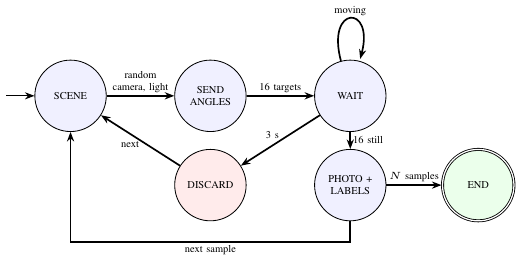
\includegraphics[width=\columnwidth]{figures/Dataset generator}
		\caption{State machine of the dataset generator. A photograph is taken only when the 16 plates report that they reached their target.}
		\label{fig:gen}
	\end{figure}
	\subsubsection{The Photograph}
	
	Four ArUco markers \cite{aruco} are placed around the module, at the height of the plates. From their centers, the photograph is \emph{rectified}: it is converted into a top view where 1~px equals 1~mm, no matter where the camera is. In that view, every plate at zero always falls on the same pixel, so a square crop of $128\times128$~px is cut around each plate. The 16 crops are what the methods receive.
	
	\vspace{1.5ex}
	\subsubsection{The Generator in Webots}
	
	Taking thousands of real photographs with known angles is not practical, so the photographs were generated in Webots \cite{webots}, where the angles are known exactly. A supervisor controller and the 16 plate controllers follow the state machine of Fig.~\ref{fig:gen}. For each sample, the supervisor chooses random angles and a random scene (camera height of 1.30--1.40~m, tilt of up to $\pm4^\circ$, yaw of up to $\pm8^\circ$, lights, and floor), sends the angles, and waits until all 16 plates report that they are still. Only then it takes the photograph and saves, as the label, the angles \emph{measured} by the joint sensors, not the commanded ones. If a plate does not arrive within 3~s, the sample is discarded. Sample~0, with every plate at zero, is the reference.
	
	\vspace{1.5ex}
	\subsubsection{The First and Second Run}
	
	Table~\ref{tab:runs} compares the two runs. The second run replaced the simplified plates with the PROTO of the real unit (generated from its CAD model with \texttt{urdf2webots} \cite{urdf2webots}), placed the units as close as possible without collisions, moved the markers closer, used five times more images, and changed how the angles are chosen: in the first run they were uniform, while in the second they follow what is expected in the robot, mostly small misalignments and sometimes large ones, as if a plate were moved by hand or jammed. In both runs the images were split \emph{by photograph} into training, validation, and test sets, so the 16 plates of one photograph never fall in different sets.
	
	\begin{table}[!t]
		\centering
		\caption{The Two Runs}
		\label{tab:runs}
		\scriptsize
		\setlength{\tabcolsep}{2pt}
		\renewcommand{\arraystretch}{1.08}
		\begin{tabularx}{\columnwidth}{@{}P{2.0cm} Y Y@{}}
			\toprule
			& First run & Second run\\
			\midrule
			Unit & Simplified plate, 69~mm, arm $L=58$~mm & Real unit (PROTO), 60~mm, arm $L=37$~mm\\
			Markers & 0.76~m square & 0.60~m square\\
			Images (train / val / test) & 2000 (1399 / 300 / 300) & 10\,000 (6999 / 1500 / 1500)\\
			Angles per plate & 5\,\% zero, 50\,\% within $\pm3^\circ$, 45\,\% within $\pm27^\circ$ & 10\,\% zero, 60\,\% up to $5^\circ$, 20\,\% 5--$15^\circ$, 10\,\% $15^\circ$--limit\\
			CNN training & 40 epochs, 84~min & 25 epochs, $\approx$4~h, in parts\\
			\bottomrule
		\end{tabularx}
	\end{table}
	
	\section{Design and Implementation of the Technological Solution}
	\label{sec:design}
	\subsection{Simulation of the 16 Module SOFIA Structure}
	
	Figure~\ref{fig2} \linelabel{ln:sim}shows the simulated response of the sixteen-module SOFIA structure while tracking the moving point. The sequence illustrates each module reorientation at different instants, where each module adjusts its two rotational degrees of freedom to maintain alignment with  reference position.
	
	\begin{figure}[!t]
		\centering
		\subfloat[Step 1]{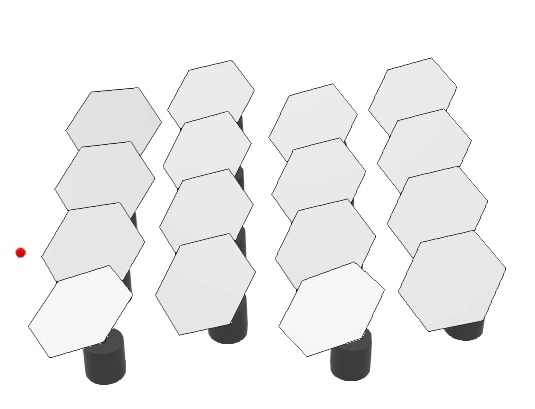
\includegraphics[width=1.1in]{figures/Sim_a}}
		\hfil
		\subfloat[Step 2]{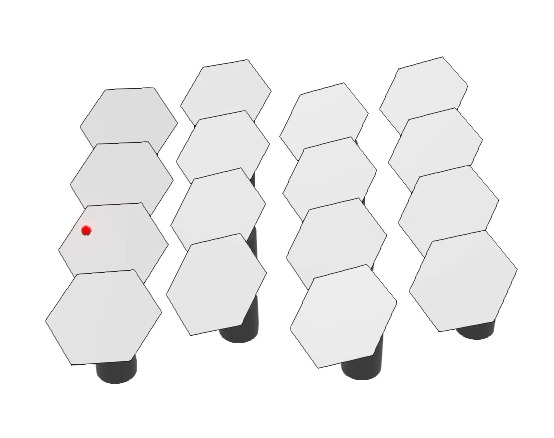
\includegraphics[width=1.1in]{figures/Sim_b}}
		\hfil
		\subfloat[Step 3]{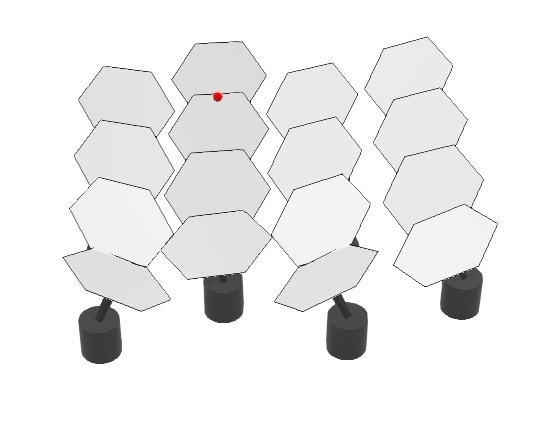
\includegraphics[width=1.1in]{figures/Sim_c}}
		\hfil
		\subfloat[Step 4]{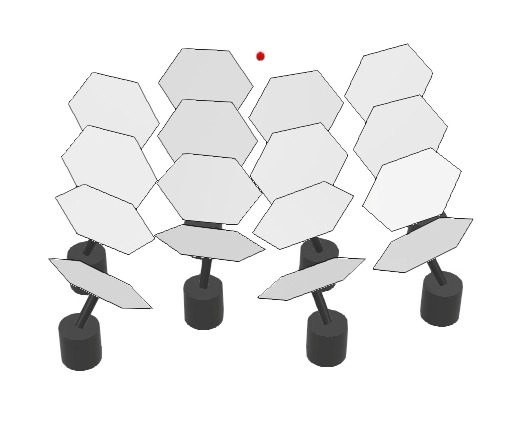
\includegraphics[width=1.1in]{figures/Sim_d}}
		\hfil
		\subfloat[Step 5]{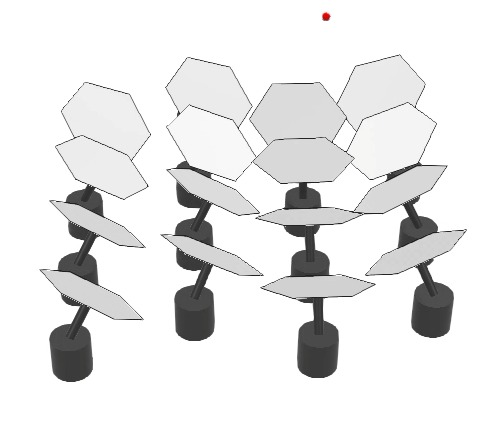
\includegraphics[width=1.1in]{figures/Sim_e}}
		\hfil
		\subfloat[Step 6]{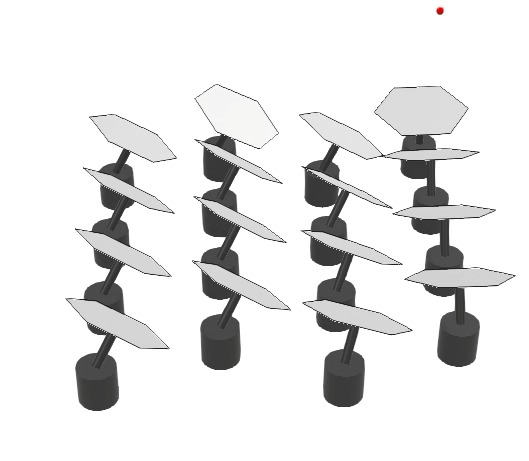
\includegraphics[width=1.1in]{figures/Sim_f}}
		\caption{Simulation of the SOFIA module tracking a moving reference point using inverse kinematics.}
		\label{fig2}
	\end{figure}
	
	Algorithm~\ref{alg:sofia_tracking} \linelabel{ln:alg}summarizes the inverse kinematics and smoothing strategy used by each SOFIA module to orient its platform toward the moving target.
	
	\begin{algorithm}[!t]
		\caption{SOFIA module target tracking control}
		\label{alg:sofia_tracking}
		
		
		\begin{algorithmic}[1]
			
			\Require Target position $\mathbf{p}$, module base position $\mathbf{r}_{0,2}$, joint limits $[q_{1\min}, q_{1\max}]$ and $[q_{2\min}, q_{2\max}]$, EMA smoothing factor $\alpha \in (0, 1]$
			\Ensure Servo command angles $q_1, q_2$
			
			\State $\mathbf{v} \gets \mathbf{p} - \mathbf{r}_{0,2}$
			\State $\hat{\mathbf{r}}_{2,p} \gets \frac{\mathbf{v}}{\|\mathbf{v}\|} = [u_x, u_y, u_z]^\top$ 
			
			\State $q_1^* \gets \operatorname{atan2}(-u_y, u_z)$
			\State $q_2^* \gets \arcsin(u_x)$ 
			
			\State $q_1^* \gets \Call{ClampAngle}{q_1^*, q_{1\min}, q_{1\max}}$
			\State $q_2^* \gets \Call{ClampAngle}{q_2^*, q_{2\min}, q_{2\max}}$
			
			\State $q_1 \gets q_{1,\text{old}} + \alpha (q_1^* - q_{1,\text{old}})$ \Comment{First-order EMA low-pass filter update}
			\State $q_2 \gets q_{2,\text{old}} + \alpha (q_2^* - q_{2,\text{old}})$
			
			\State Apply $q_1, q_2$ to servo motors
			
			\State \Return $q_1, q_2$
			
		\end{algorithmic}
	\end{algorithm}
	
	\subsection{Mechanical assembly}
	\linelabel{ln:cad}The mechanical assembly was documented using an exploded
	view generated in SolidWorks, as shown in
	Fig.~\ref{fig:sofia_expl_cad}. The drawing illustrates
	the arrangement of the structural components,
	joint mechanisms, and fastening elements, while the
	accompanying bill of materials identifies their
	part numbers and quantities.
	
	\begin{figure}[!t]
		\centering
		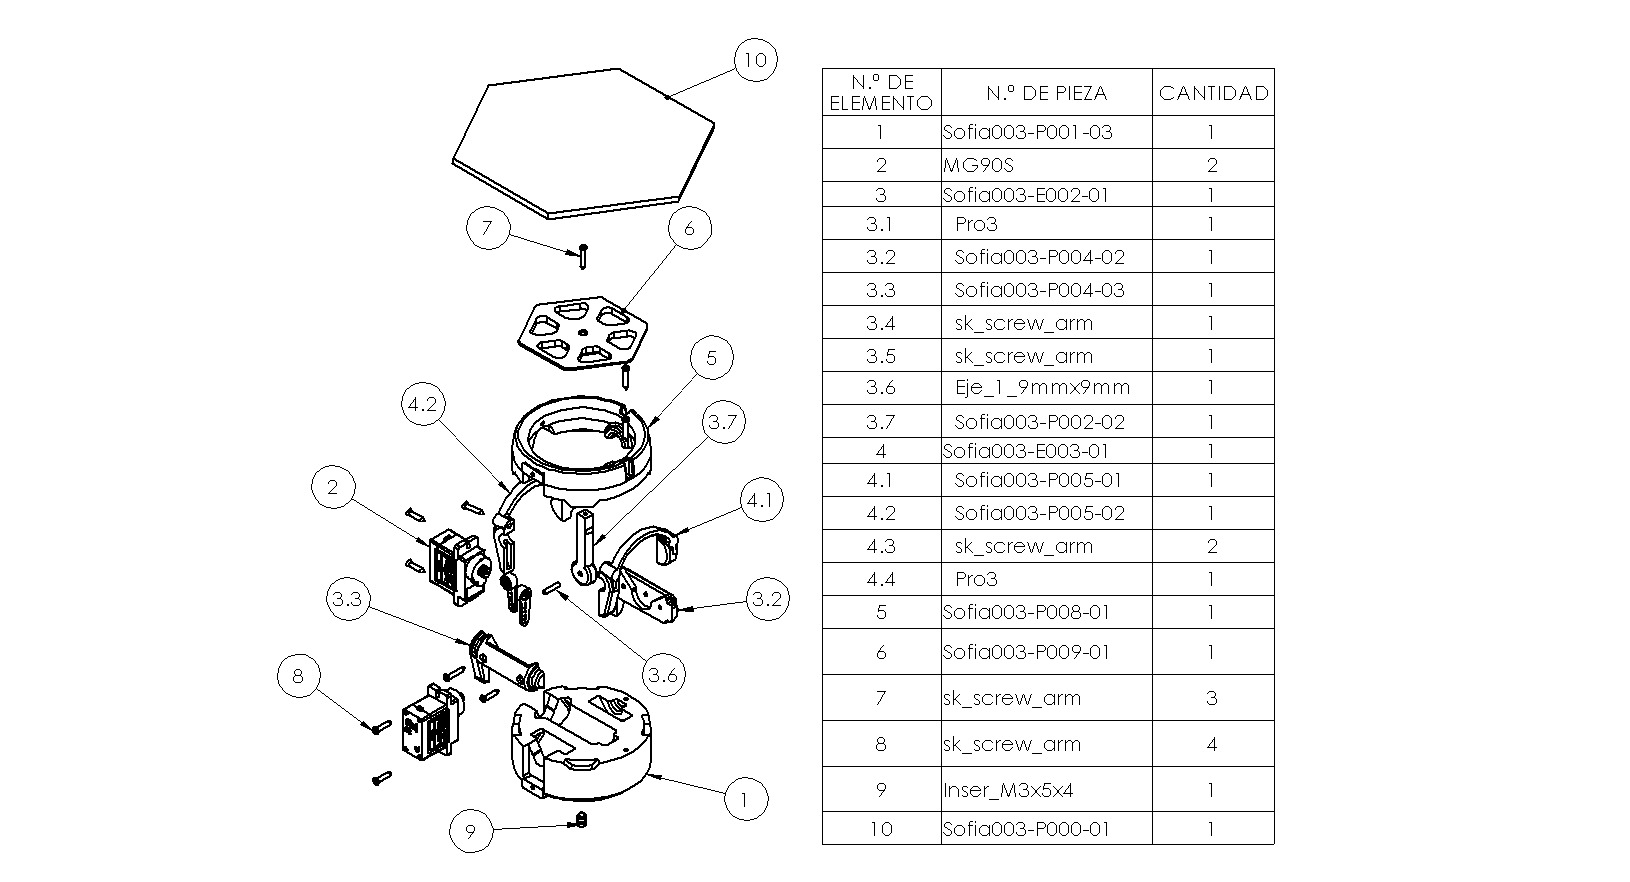
\includegraphics[width=\columnwidth, trim={2cm, 0, 5cm, 0},]{figures/sofia_expl_cad.jpg}
		\caption{Exploded assembly drawing of the SOFIA electromechanical module, including component identification.}
		\label{fig:sofia_expl_cad}
	\end{figure}
	
	\subsection{Methods and Training of the Vision-Based Misalignment Diagnosis}
	
	\subsubsection{Geometric Method}
	
	It finds each plate in the top view and measures how far its center moved from the reference. With the plate at a distance $L$ from the joint axes, the shift is $\Delta v = L\sin\theta_2$ and $\Delta u = L\cos\theta_2\sin\theta_1$, which gives the two angles directly. It needs no training, but an error of 1~mm in the position becomes an error of $1/L$ radians: $1.0^\circ$ with $L=58$~mm and $1.5^\circ$ with $L=37$~mm.
	
	\vspace{1.5ex}
	\subsubsection{CNN}
	
	A small CNN (five blocks of convolutions, 1.28~M parameters) receives one crop and returns the two angles. It was trained in PyTorch \cite{pytorch} with the training images, mirrored and with random changes of light and noise so that it does not depend on a single scene. After every epoch, its error is measured on the validation images, and only the best epoch is kept. The test images are used once, at the end, to report the results.
	
	Since the second run takes about 4~hours, training was split into sessions with the state machine of Fig.~\ref{fig:train}. The complete state (weights, optimizer, and learning rate) is saved after every epoch, so a session can stop after a time limit or with Ctrl+C and the next one resumes at the same epoch, as if it had not stopped.
	
	\begin{figure}[!t]
		\centering
		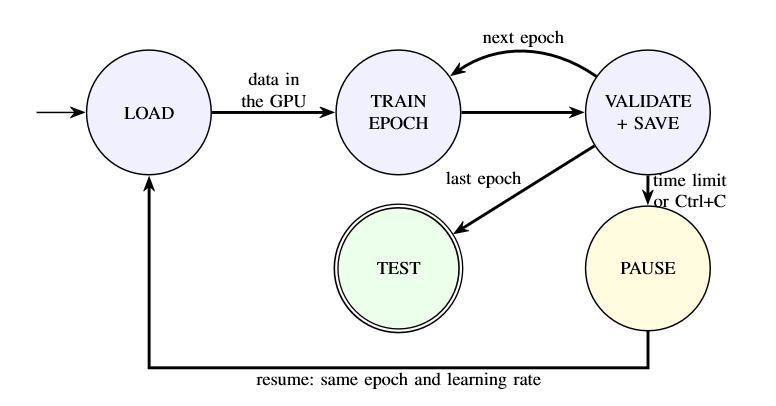
\includegraphics[width=\columnwidth]{figures/State_machine_training}
		\caption{State machine of the training. The state is saved after every epoch, so training can be split into several sessions.}
		\label{fig:train}
	\end{figure}
	
	\vspace{1.5ex}
	\subsubsection{Hybrid Rule}
	
	Both methods are run, and for each plate: if they differ by more than $2^\circ$, the CNN is used and the plate is marked for inspection; if they agree and the plate is near zero ($\le6^\circ$), the geometric value is used; otherwise, the CNN. It was designed in the first run, where the geometric method was the most accurate near zero.
	
	\vspace{1.5ex}
	\subsubsection{Why ResNet18 Was Dropped}
	
	In the first run, a ResNet18 \cite{resnet} pretrained on ImageNet was also trained. Although it is ten times larger (13.3~M parameters), it was less accurate than the small CNN (Table~\ref{tab:results_Vision_Train}): what it learned from everyday photographs does not help to measure a shift of a few pixels. For this reason, and to save training time, it was not used in the second run.
	
	\subsection{Computer Vision Gesture Recognition System Architecture}
	
	\linelabel{ln:intro-vis}The computer vision subsystem of SOFIA recognizes human gestures in real time and translates them into discrete action labels. Using a webcam, the modular Python application captures user movements to establish a gesture-based interaction method for future integration with the robot's control and actuation systems.
	
	\linelabel{ln:explain-vis}The implementation combines OpenCV for image acquisition and visualization with MediaPipe Tasks for landmark detection. It utilizes two pretrained models—Pose Landmarker (33 body landmarks) and Hand Landmarker (up to two hands with 21 landmarks each)—bypassing custom neural network training by classifying gestures through predefined geometric rules.
	
	\linelabel{ln:model-vis}Organized within the \texttt{Vision/} directory, the modular architecture uses \texttt{main.py} to orchestrate frame capture, model execution, evaluation, and visualization. Landmark detection is handled by \texttt{pose\_detector.py} and \texttt{hand\_detector.py}, while \texttt{gesture\_detector.py} performs classification using \texttt{geometry\_utils.py} for geometric calculations and \texttt{smoothing.py} for temporal stabilization.
	
	\linelabel{ln:model-vis2}Captured BGR frames are converted to RGB for MediaPipe processing. Body landmarks are filtered via an Exponential Moving Average (EMA) to reduce frame-to-frame fluctuations, enabling the system to evaluate normalized distances, joint angles, and relative positions. Hand landmarks are concurrently analyzed to identify specific finger configurations.
	
	\linelabel{ln:model-vis3}The system recognizes five gestures divided into dynamic gestures (START and END, requiring movement sequences over time) and static gestures (RELOAD, SHIELD, and ATTACK, defined by specific body and hand configurations). Once recognized, the interface displays the gesture label, detected landmarks, and a real-time frames-per-second (FPS) indicator.
	
	\linelabel{ln:model-vis4}The perception subsystem is integrated with the ESP32-C3 controller over wireless telemetry, translating recognized gestures into coordinated actuation commands across the 16 physical modules.
	
	\subsection{Geometric Gesture Recognition}
	
	\linelabel{ln:Geo-ges-rec-intro}The gesture recognition system was designed to identify five predefined human gestures through geometric analysis of body and hand landmarks. Instead of training a custom classification model, the implementation uses deterministic rules based on normalized distances, joint angles, relative positions, and movement sequences. This approach allows each gesture to be defined through specific conditions while keeping the recognition process modular and interpretable.
	
	\linelabel{ln:Geo-ges-rec2}To reduce the influence of the user's distance from the camera, several geometric measurements are normalized using anatomical references, such as shoulder width and torso height. The normalized distance between two landmarks is calculated as:
	\begin{equation}
		D_{\text{norm}} = \frac{\sqrt{(x_A - x_B)^2 + (y_A - y_B)^2}}{d_{\text{ref}}}
	\end{equation}
	where $A$ and $B$ represent the selected landmarks, and $d_{\text{ref}}$ is the distance between two anatomical reference points.
	
	\linelabel{ln:Geo-ges-rec3}For gestures involving arm positioning, joint angles are calculated using three landmarks. The angle between two vectors, with the elbow as the central point, is defined as:
	\begin{equation}
		\theta = \cos^{-1}\left( \frac{\mathbf{u} \cdot \mathbf{v}}{\|\mathbf{u}\| \|\mathbf{v}\|} \right)
	\end{equation}
	\linelabel{ln:Geo-ges-rec4}These angles are calculated from the two-dimensional projection of the detected landmarks and are used to evaluate arm configurations.
	
	\linelabel{ln:Geo-ges-rec5}The five gestures are divided into two dynamic gestures and three static gestures, depending on whether recognition requires a movement sequence or a specific body configuration described in Table~\ref{tab:gesture_conditions}.
	
	\begin{table}[!t]
		\centering
		\caption{Summary of Gesture Recognition Conditions}
		\label{tab:gesture_conditions}
		\vspace{0.5em}
		\begin{tabularx}{\columnwidth}{@{}c l X@{}}
			\toprule
			\textbf{Gesture} & \textbf{Type} & \textbf{Main recognition conditions} \\
			\midrule
			START & Dynamic & Three wrist-to-hip contacts within 3s \\
			END & Dynamic & One raised hand and two horizontal direction changes \\
			RELOAD & Static & Wrists near shoulders, approximately vertical forearms, no two recognized pistol hands \\
			SHIELD & Static & Crossed arms, wrists near opposite shoulders, elbow below shoulders \\
			ATTACK & Static & Elbow angles of 35$^\circ$--125$^\circ$ and two pistol-shaped hands \\
			\bottomrule
		\end{tabularx}
	\end{table}
	
	\linelabel{ln:vision-evaluation}The system evaluates these conditions using the body landmarks estimated by MediaPipe Pose Landmarker and the finger landmarks provided by MediaPipe Hand Landmarker. The resulting geometric conditions are used to determine the recognized gesture, while temporal confirmation mechanisms are applied to improve the stability of static gesture classification.
	
	\subsection{Temporal Filtering and Gesture Validation}
	
	To optimize stability, an Exponential Moving Average (EMA) filter is applied to body landmarks using the next equation: 
	\begin{equation}
		S_t = \alpha X_t + (1 - \alpha)S_{t-1}
	\end{equation} 
	implemented with $\alpha = 0.3$ resulting in:
	\begin{equation}
		S_t = 0.3X_t + 0.7S_{t-1}
	\end{equation} 
	
	\linelabel{ln:five-frame}Additionally, static gestures require a five-consecutive-valid-frame confirmation, and the system manages display priorities during simultaneous activations by prioritizing SHIELD, ATTACK, RELOAD, START, and END.
	
	\subsection{Integration Challenges and Design Refinements}
	
	\linelabel{ln:chal-intro}During development, challenges in landmark stability, gesture overlap, and software integration prompted targeted algorithmic and architectural revisions. To prevent \texttt{AttributeError} crashes when users left the camera frame, missing-landmark validation was added prior to processing. Coordinate fluctuations near recognition thresholds were mitigated by incorporating an EMA filter ($\alpha = 0.3$) alongside a 5-consecutive-frame static confirmation requirement.
	
	\linelabel{ln:chal-reload}RELOAD was converted from a dynamic gesture to a static posture (bent arms, hands near shoulders), refined with constraints on wrist-to-shoulder proximity, vertical bounds, and vertical forearm orientation. 
	To resolve spatial overlap with ATTACK, RELOAD classification is suppressed whenever both hands are detected in a pistol configuration. ATTACK itself was redefined—discarding strict torso proximity, depth restrictions, and an ineffective $90^\circ$–$165^\circ$ elbow range—in favor of a W-shaped posture requiring elbow angles between $35^\circ$ and $125^\circ$, wrists above elbows, and outward hand orientation.
	
	\subsection{PCB Design and Electronic Integration}
	\label{subsec:pcb_design}
	
	\linelabel{ln:pcb}
	A single-layer printed circuit board (PCB)
	was developed as a functional integration
	prototype for the SOFIA modular kinetic
	surface. The board provides the electrical
	interconnections and mounting interfaces
	for an ESP32-C3 SuperMini, two PCA9685
	PWM driver modules, and MAX13487E RS-485
	communication interfaces, as illustrated
	in Fig.~\ref{fig:sofia_schematic}.
	
	The ESP32-C3 communicates with both PCA9685
	modules through the I2C bus, providing
	32 PWM channels for servomotor control.
	The servomotors are powered by an external
	5 V supply, while the RS-485 interfaces
	are intended to support future inter-module
	communication. A resistive voltage divider
	consisting of 10 kOhm and 20 kOhm resistors
	reduces the nominal 5 V receiver output
	of the RS-485 transceiver to approximately
	3.33 V at the microcontroller input.
	
	
	\begin{figure*}[!t]
		\centering
		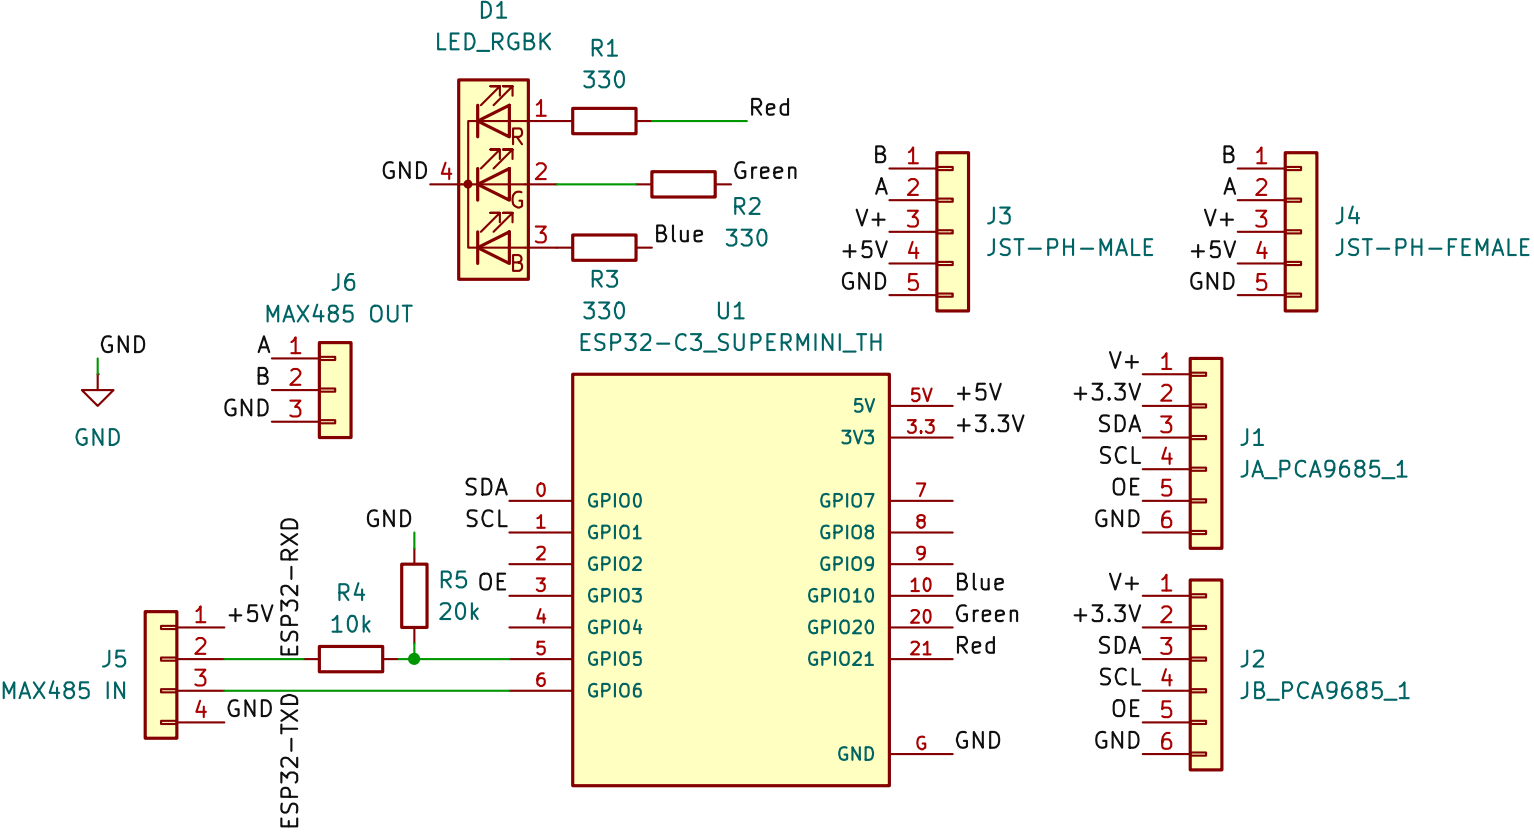
\includegraphics[width=\textwidth]
		{figures/sofia_pcb_schematic.png}
		\caption{Revised electronic schematic of
			the SOFIA control PCB.}
		\label{fig:sofia_schematic}
	\end{figure*}
	
	\linelabel{ln:pcb-traces}
	The PCB layout was developed with 0.7 mm-wide
	traces for power distribution and 0.5 mm-wide
	traces for signal routing. The component
	arrangement, copper routing, and overall
	board dimensions are illustrated in
	Fig.~\ref{fig:sofia_pcb}.
	
	\begin{figure*}[!t]
		\centering
		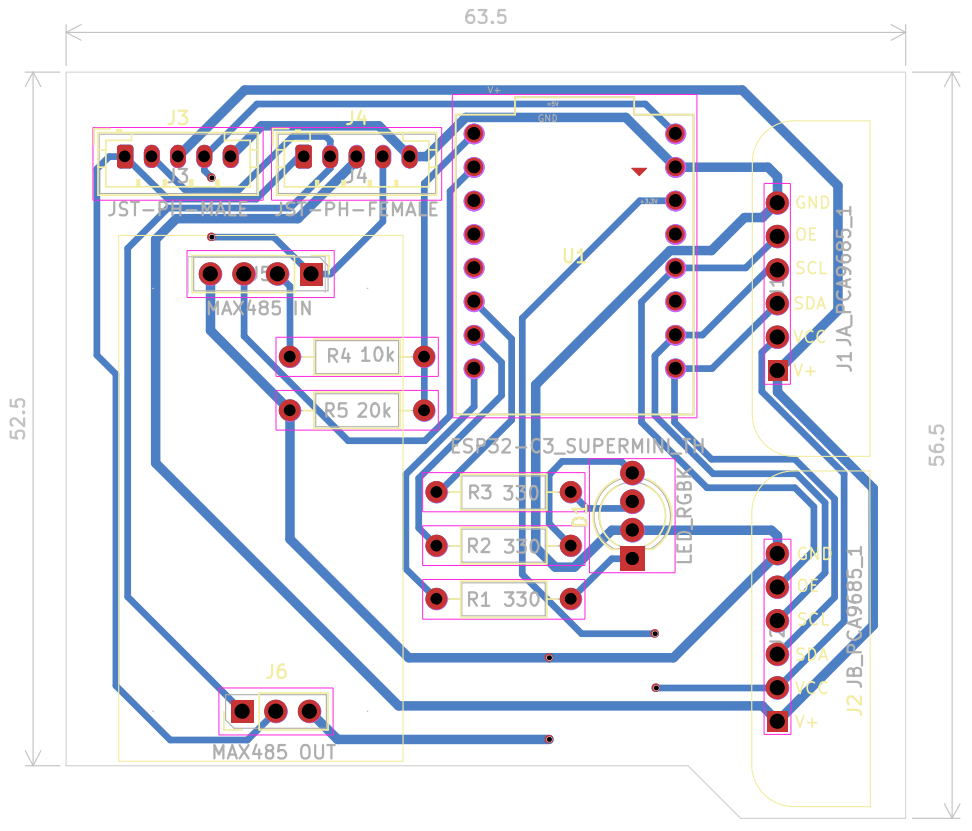
\includegraphics[width=\textwidth]
		{figures/sofia_pcb.png}
		\caption{Single-layer PCB prototype showing
			component placement, copper routing,
			and board dimensions.}
		\label{fig:sofia_pcb}
	\end{figure*}
	
	\subsection{PCB Prototype Limitations}
	\linelabel{ln:pcb-revision}
	The PCB was developed as a functional
	prototype for integrating the SOFIA
	electronic subsystems. However, its
	current-carrying capacity and power
	distribution performance have not yet
	been validated under full system load.
	
	Future work will focus on characterizing
	servomotor current consumption, verifying
	PCB trace and connector ratings, and
	evaluating power distribution and
	decoupling requirements to support
	reliable operation of the complete system.
	
	
	\section{Results}
	\label{sec:results}
	
	\subsection{Preliminary Servomotor Dynamic Response}
	\linelabel{ln:speed}Preliminary speed profiling was conducted on a single module across 12 setpoints ($30^\circ/\text{s}$ to $600^\circ/\text{s}$). The servomotors demonstrated smooth trajectory execution at low-to-medium velocities ($30^\circ/\text{s}$--$350^\circ/\text{s}$). Beyond $500^\circ/\text{s}$, little mechanical chatter and motion desynchronization occurred, establishing $350^\circ/\text{s}$ as the maximum operational threshold for smooth servo motor actuation.
	
	\subsection{Results for the Training Methods of Vision-Based Misalignment Diagnosis}
	
	Table~\ref{tab:results_Vision_Train} shows the error on the test images of each run (300 and 1500 photographs). The two test sets are not the same, since the unit and the distribution of angles changed, so the comparison is between the two complete setups.
	
	\begin{table}[!t]
		\centering
		\caption{Test Error ($^\circ$) and State Accuracy}
		\label{tab:results_Vision_Train}
		\scriptsize
		\setlength{\tabcolsep}{2.5pt}
		\renewcommand{\arraystretch}{1.08}
		\begin{tabularx}{\columnwidth}{@{}Y c c c c c@{}}
			\toprule
			Method & Mean & Max & $0$--$5^\circ$ & $>15^\circ$ & States\\
			\midrule
			\multicolumn{6}{@{}l}{\textit{First run (simplified plates, 2000 images)}}\\
			Geometric & 0.539 & 74.0 & \textbf{0.13} & 1.30 & 97.2\,\%\\
			CNN & 0.248 & 4.4 & 0.18 & \textbf{0.36} & 96.3\,\%\\
			ResNet18 & 0.293 & 4.1 & 0.21 & 0.43 & 95.9\,\%\\
			Hybrid & \textbf{0.223} & 4.4 & \textbf{0.13} & \textbf{0.36} & \textbf{97.2\,\%}\\
			\midrule
			\multicolumn{6}{@{}l}{\textit{Second run (real unit, 10\,000 images)}}\\
			Geometric & 0.521 & 5.9 & 0.33 & 1.60 & 94.1\,\%\\
			CNN & \textbf{0.204} & \textbf{3.3} & \textbf{0.17} & \textbf{0.41} & \textbf{96.8\,\%}\\
			Hybrid & 0.329 & \textbf{3.3} & 0.33 & \textbf{0.41} & 94.1\,\%\\
			\bottomrule
		\end{tabularx}
	\end{table}
	
	\textbf{First run.} Each method was good at something different. The geometric method was the most precise near zero ($0.13^\circ$), but sometimes failed badly (up to $74^\circ$) when a very tilted plate was confused with its neighbor. The CNN never failed badly (at most $4.4^\circ$). The hybrid rule took the best of both and was the best method ($0.223^\circ$).
	
	\textbf{Second run.} The CNN improved to $0.204^\circ$ with an error of at most $3.3^\circ$ in 24\,000 plates, and became the best method in every range, even near zero. The geometric method lost precision near zero ($0.13^\circ \rightarrow 0.33^\circ$) because the arm of the real unit is shorter, so the plate moves less per degree and each pixel of error weighs more; on the other hand, it no longer fails badly (at most $5.9^\circ$). As a consequence, the hybrid rule \emph{fell} from the best to the middle ($0.329^\circ$): it uses the geometric value precisely near zero, where it is now the least precise. Its inspection marks are not useful either: 873 of its 901 marks were errors of the geometric method, not of the CNN. The CNN is therefore the default method; the geometric method remains as a fallback without a GPU.
	
	Two lessons follow. First, more and more realistic images made the CNN better, even with a harder unit. Second, a CNN must be retrained when the unit changes: the CNN of the first run, tested on the real unit, had an error of $1.6^\circ$.
	
	\subsection{Functional Validation of the Vision Gesture Recognition Subsystem}
	
	\linelabel{ln:res-func-intro}The computer vision subsystem was tested through real-time webcam experiments to verify its ability to recognize the five predefined gestures. The tests focused on body and hand landmark detection, geometric gesture classification, and temporal validation.
	
	\linelabel{ln:vision-vis}The system successfully captured and processed video frames using OpenCV and MediaPipe, displaying the detected landmarks, recognized gesture labels, and approximate FPS in real time.
	
	\linelabel{ln:vision-func-tests}Functional tests confirmed the recognition of START through three consecutive hand-to-thigh movements and END through two horizontal direction changes of a raised hand. For static gestures, SHIELD was recognized through crossed-arm positioning, RELOAD through the defined arm configuration near shoulder height, and ATTACK through the combination of W-shaped arms and two pistol-shaped hands.
	
	\linelabel{ln:vision-func-ema}The implementation of EMA filtering and five-frame temporal confirmation maintained the functionality of the recognition system while providing mechanisms to reduce unstable detections. Additionally, the final adjustments to RELOAD and ATTACK were verified, confirming that the updated gesture definitions could be recognized during functional testing.
	
	\linelabel{ln:vision-func-summary}These results demonstrate the functional operation of the five-gesture recognition subsystem as an independent software prototype. However, recognition accuracy, average response time, and robustness under different environmental conditions still require quantitative evaluation.
	
	\subsection{Gesture Recognition Performance Evaluation}

	\linelabel{ln:res-vision-intro}Preliminary performance tests
	were conducted with three participants under adequate lighting
	conditions and at a comfortable distance from the webcam.
	The exact distance and illumination levels were not recorded.
	These tests evaluated an earlier version of the gesture
	recognition system and recorded the expected gesture, detected
	gesture, response time, and instantaneous frames per second
	(FPS).

	\linelabel{ln:vision-performance}As shown in
	Table~\ref{tab:gesture_benchmark}, 42 out of 50 attempts were
	correctly recognized, resulting in an overall accuracy of
	84.0\%. Dynamic gestures (START and END) achieved 100\%
	recall, while static gestures achieved recall values between
	75.0\% and 88.9\%. Wilson confidence intervals at the 95\%
	level were calculated assuming independent trials.

	\begin{table}[!t]
		\centering
		\caption{Preliminary Gesture Recognition Performance}
		\label{tab:gesture_benchmark}
		\scriptsize
		\setlength{\tabcolsep}{3pt}
		\renewcommand{\arraystretch}{1.1}
		\begin{tabular}{@{}l c c c c c@{}}
			\toprule
			\textbf{Gesture} &
			\textbf{Trials} &
			\textbf{Hits} &
			\textbf{Recall (\%)} &
			\textbf{95\% CI (\%)} &
			\textbf{Resp. (s)} \\
			\midrule
			START  & 6  & 6  & 100.0 & 61.0--100 & 1.33 \\
			RELOAD & 9  & 8  & 88.9  & 56.5--98.0 & 4.17 \\
			SHIELD & 12 & 9  & 75.0  & 46.8--91.1 & 1.06 \\
			ATTACK & 16 & 12 & 75.0  & 50.5--89.8 & 1.14 \\
			END    & 7  & 7  & 100.0 & 64.6--100 & 0.95 \\
			\bottomrule
		\end{tabular}
	\end{table}

	\linelabel{ln:vision-shield}During an initial evaluation of
	SHIELD, two out of four attempts were correctly classified,
	while the remaining two were incorrectly identified as RELOAD.
	The relationship between these four attempts and the 50-trial
	evaluation could not be verified.

	\linelabel{ln:vision-overlap}These preliminary observations
	helped identify overlapping recognition conditions, leading
	to refinements in the geometric classification rules.

	\linelabel{ln-vision-latency}The recorded response times
	included user reaction, gesture execution, and software
	processing. Therefore, they do not represent the algorithm's
	computational latency alone.

	\linelabel{ln:vision-adjustments}Following these observations,
	the recognition conditions for RELOAD and ATTACK were adjusted
	and their functionality was verified. However, individual
	trial records were unavailable to reconstruct a complete
	confusion matrix, preventing reliable calculation of
	precision and F1-score. The limited number of participants
	and potentially dependent trials also restrict the
	generalizability of the results. Quantitative validation
	of the final implementation remains pending.

		
	\section{Discussion}
	\label{sec:discussion}

	The preliminary gesture recognition results demonstrate the
	feasibility of geometric classification for human-robot
	interaction, achieving an overall accuracy of 84.0\%.
	Dynamic gestures showed higher recall than static gestures
	in the evaluated trials. However, the limited sample size,
	overlapping recognition conditions, and wide confidence
	intervals restrict the generalization of these results.

	The electronic architecture supports the integration of
	visual perception and servomotor control. Nevertheless,
	the current-carrying capacity of the PCB and the electrical
	performance of the revised design require further
	experimental validation.

	The implementation of vision-based orientation correction
	introduces external feedback to the SOFIA control system,
	allowing adjustments based on the estimated physical
	orientation of the platforms. Its effectiveness in reducing
	angular deviations remains to be quantified through
	experimental comparison.

	
	
	\section{Conclusions}
	\label{sec:conclusions}

	The development of SOFIA integrates mechanical actuation,
	embedded control, and computer vision into a modular
	robotic platform. Preliminary gesture recognition tests
	achieved an overall accuracy of 84.0\%, demonstrating
	the potential of geometric classification for human-robot
	interaction.

	The implementation of a vision-based orientation estimation
	and correction system enables automatic servomotor
	adjustments using external visual feedback. This approach
	establishes a means of addressing deviations between
	commanded and actual platform orientations. Further
	experimental validation is required to quantify angular
	estimation accuracy, correction performance, and the
	effectiveness of the integrated control system.

	
	\balance
	
	\bibliographystyle{IEEEtran}
	\bibliography{bibliography}
	
\end{document}